\documentclass{vgtc}

\ifpdf%                                % if we use pdflatex
\pdfoutput=1\relax                   % create PDFs from pdfLaTeX
\pdfcompresslevel=9                  % PDF Compression
\pdfoptionpdfminorversion=7          % create PDF 1.7
\ExecuteOptions{pdftex}
\usepackage{graphicx}                % allow us to embed graphics files
\DeclareGraphicsExtensions{.pdf,.png,.jpg,.jpeg} % for pdflatex we expect .pdf, .png, or .jpg files
\else%                                 % else we use pure latex
\ExecuteOptions{dvips}
\usepackage{graphicx}                % allow us to embed graphics files
\DeclareGraphicsExtensions{.eps}     % for pure latex we expect eps files
\fi%

\usepackage{booktabs} % For formal tables
\usepackage{color, soul}
\usepackage{hyperref}
\usepackage{url}
\def\UrlBreaks{\do\/\do-}
\graphicspath{{figures/}}
\usepackage{amsthm}
\theoremstyle{definition}
\newtheorem{definition}{Definition}[section]
\usepackage{subcaption}
\usepackage{graphicx}
\usepackage[]{units}

\abstract{Yelp is a crowd-sourced local business review and social networking community, which has hundreds of thousands of users contribute their data every day. Based on users' reviews and ratings, good local businesses stand out among their categories on top of the list, acting as a word-of-mouth reference. However, tons of user data doesn't make any sense unless we make good use of it. In this case, we decided to look into the problem that how we might get as much as useful information from our data with a particular interest in how the users' rating behavior are influenced by different factors, and what kind of prediction we can make out of the rating pattern we found. With various features extracted from Yelp data, we conducted feature selection, best split and finally built a Decision Tree model which predicts users' rating based on those features. Our visualization includes the complete process of this typical machine learning method, which provides insights about the inner mechanism of how the rating prediction is conducted. }

\begin{document}
\title{Yelp Rating Prediction Visualization}

\author{Jiawen Liu\thanks{e-mail: Jiawen Liu}\\ %
	\and Keke Wu\thanks{e-mail: Keke.Wu@colorado.edu}\\ %
	\and Wei Miao\thanks{e-mail: Wei.Miao@colorado.edu}\\ %
	\and Xu Han\thanks{e-mail: Xu.Han@colorado.edu}\\ %
	\and Yawen Zhang\thanks{e-mail: Yawen.Zhang@colorado.edu}\\ %
	}

%\author{Jiawen Liu}
%\email{Jiawen Liu}
%
%\author{Keke Wu}
%\email{Keke.Wu@colorado.edu}
%
%\author{Wei Miao}
%\email{Wei.Miao@colorado.edu}
%
%\author{Xu Han}
%\email{Xu.Han@colorado.edu}
%
%\author{Yawen Zhang}
%\email{Yawen.Zhang@colorado.edu}

%\author{Charles Palmer}
%\affiliation{%
%  \institution{Palmer Research Laboratories}
%  \streetaddress{8600 Datapoint Drive}
%  \city{San Antonio}
%  \state{Texas} 
%  \postcode{78229}}
%\email{cpalmer@prl.com}

%\begin{abstract}

\textcolor{red}{Your motivating problem, what you did, and what you found}

Yelp is a crowd-sourced local business review and social networking community, which has hundreds of thousands of users contribute their data every day. Based on users' reviews and ratings, good local businesses stand out among their categories on top of the list, acting as a word-of-mouth reference. However, tons of user data doesn't make any sense unless we make good use of it. In this case, we decided to look into the problem that how we might get as much as useful information from our data with a particular interest in how the users' rating behavior are influenced by different factors, and what kind of prediction we can make out of the rating pattern we found. With various features extracted from Yelp data, we conducted feature selection, best split and finally built a Decision Tree model which predicts users' rating based on those features. Our visualization includes the complete process of this typical machine learning method, which provides insights about the inner mechanism of how the rating prediction is conducted. 

\end{abstract}

 

%\keywords{Yelp; Rating Prediction; Decision Tree}

\maketitle

\section{Introduction}
\label{sec:intro}

\textcolor{red}{The motivating Problem, why it's interesting or important}

Rating prediction plays an important role in the recommendation system as to capture users' preference for specific product. In Yelp, user can post their rating and review for a restaurant they visited, and these data as well as user/restaurant related attributes, e.g., user average rating, restaurant location or category, can be well gathered for conducting the rating prediction. If a user's rating for a restaurant can be accurately predicted, Yelp would be able to recommend high rating product to the user which meets their preferences. 

The challenge in this problem lies in the feature selection and modeling processing. With multiple features related to a user's rating, picking up the effective features is quite important, which would significantly influence the prediction performance. Additionally, the modeling process which selects the best machine learning model for rating prediction is also critical, and it's necessary to gain insights about how the model functions, i.e., the inner mechanism of model. Previously, most machine learning processes have been conducted in a "black box", by just showing input and output. In our project, we aim at visualizing the whole process, including feature selection, best split, and model tree. The Decision Tree model is selected because its straightforward idea in classification, which would be beneficial for visualization. 

\section{Related Work}
\label{sec:related} 

%\textcolor{red}{Summarize research related to your projects, minimum 8 citations. }

In this project, we deploy the visualization principles and techniques to make mechanism of the whole recommendation system(RS) transparent based on Yelp's public dataset\cite{}. A lot of research has been done on recommendation system and the RS techniques are broadly divided into two types: memory-based approach, which recommend business based on similarity or correlation between users\cite{}, and model-based approach, which use machine learning methods to predict user ratings\cite{}. In our project, we use decision tree from model-based approach\cite{} as our visualization example. 

Our visualization of modeling process mainly focus on four parts: feature engineering, best split analysis, feature ranking and model training. For feature engineering, we extract 22 features in total, includes user-related features(7), business-related features(3), user-category features(5) and review-related features(7). Among review-related features, we extract several advanced natural language processing(NLP) features like polarity\cite{} and subjectivity\cite{}. For best spllit analysis, we create a moveable threshold to study how this feature -- business average star, could influence the decision making(whether to recommend or not). When moving the threshold, the calculated accuracy and true positive rate\cite{} will be changed correspondingly and we can choose the threshold with highest accuracy as our decision tree's best split. In the part of feature ranking, we measure the importance of all 22 features based on the score retrieved by Xgboost\cite{}. Xgboost's feature importance method calculateds F score, which indicates how many times the feature split on. Higher the F score is, more important the feature is. In our feature ranking visualization, we use a radar graph to show the importance of all these features based on F score. The last step is model training, we use 100 users as an example. 80 users are used to train and 20 users are used to test. The top three features with highest F score are selected and used by the model. We visualize each users path and the overall test accuracy.
\section{Design Process}
\label{sec:design} 

%\textcolor{red}{Justifications for any design elements}

During the design process, we tried to get our results displayed in a reader-driven rather than author-driven way, following a storytelling style. Our preliminary works included data cleaning, data organization by categories, feature selection, hand-written sketches of the complete workflow. We used web as our platform and D3.js as the main tool. The web was divided into six different but consistent sections in the order of Our Story, Our Goal, Our Design, Visualization, Split and Tree Model, which was exactly the sequence we were following to dive into this topic. In terms of the visual design, we used the red, black and white color scheme adopted by Yelp to make it look consistent. Besides text descriptions and interactive visualization graphs, we also had hand-written sketches on the web as a proof of concept, which helped enrich the design elements' diversity. In terms of the visualization design, we used four different types of charts to visualize four different rating related data features. The restaurant ratings by category were visualized in a bar chart, showing customers' preferences on cuisines. The average ratings by state were visualized in a US map, with the darker colored state having a higher rating trend. We also extracted key words from users' reviews and got them displayed in a randomly generated word cloud, where the words were extinguished from each other by five colors mapped with five different rating stars. Besides these, we also built a network to visualize the influence on ratings from Yelp users who have most friends. All of these charts were interactive and dynamic, enabling a good user-directed exploration experience. Following sections utilized a split framework to explain how we applied machine learning to help us make predictions. Finally, a decision-tree like model walked the audience through the decision and prediction making process. With a well-designed and fully-interactive design style, we hope to help our audience get valuable information in a way that can be adjusted as they like. Meanwhile, we hope to use some vivid graphs and animations to bridge the gap between scientific research and general public understanding, making the abstract concept intuitive and straightforward.

\section{Modeling Process}
\label{sec:modeling} 

%\textcolor{red}{Decision Tree}

For Yelp rating prediction, we use Decision Tree, which is tree-like graph of decisions and their possible consequences. It is widely used prediction model in machine learning. In this tree structure, leaves represent class labels and branches represent conjunctions of features that lead to the class labels. A typical example is shown in Figure \ref{fig:DT} \footnote{\url{https://en.wikipedia.org/wiki/Decision_tree_learning}}. The modeling process include feature selection, best split, feature ranking and tree generation. 

%-------------------------------------------
\begin{figure}[h]
	\centering
	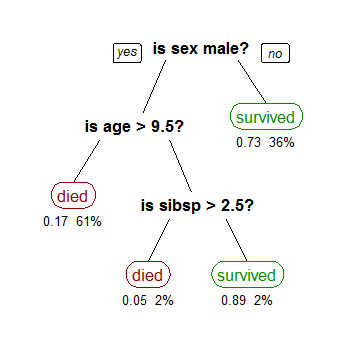
\includegraphics[width=6cm]{DT.png}
	\caption{A Decision Tree showing survivals of passengers of the Titanic.}
	\label{fig:DT}
\end{figure}
%------------------------------------------- 


\paragraph{Feature Selection}
%There are multiple features related a user's rating. \textcolor{red}{give list or table, showing all features. }
Yelp dataset contains 11 tables such as Yelp dataset contains 11 tables such as business, category, checkin, etc. Figure \ref{fig:data}\footnote{\url{https://www.yelp.com/dataset/documentation/sql}} shows the dataset structure. We extract 22 features(shown in Table \ref{tb:feature}, which could be divided into four groups: user-related features(7), business-related features(3), user-category features(5) and review-related features(7).

%-------------------------------------------
\begin{figure}[h]
	\centering
	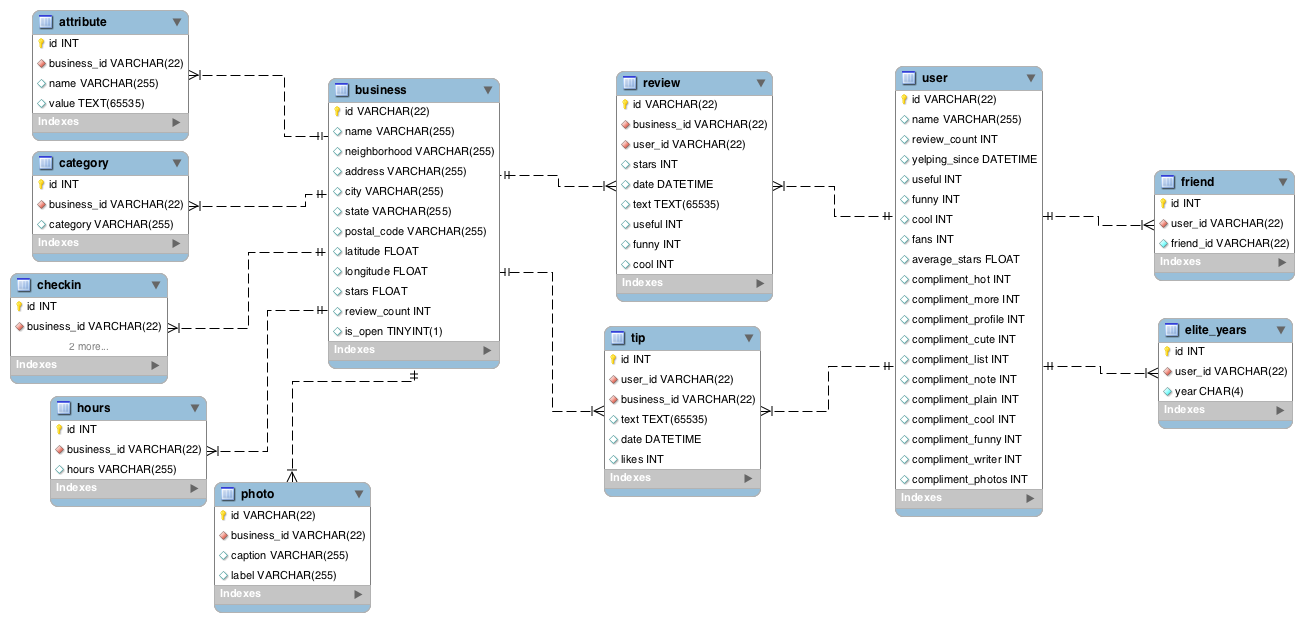
\includegraphics[width=6cm]{data.png}
	\caption{The structure of Yelp Dataset}
	\label{fig:data}
\end{figure}
%------------------------------------------- 
\newcommand{\tabincell}[2]{\begin{tabular}{@{}#1@{}}#2\end{tabular}}
\begin{table}
\centering
\caption{Feature Groups}
\label{table:para_regression}
\begin{tabular}{|c|c|}
\hline
Feature Group & Features \\ \hline
User-related Features(7) & \tabincell{c}{user compliment count\\user funny count\\user cool count\\user useful count\\user fans count \\ user review count \\ user average rating} \\ \hline
Business-related Features(3) & \tabincell{c}{business average rating\\business location-related rating\\business neighborhood-related rating} \\ \hline
Review-related Features(7) & \tabincell{c}{Polarity \\  Subjectivity  \\  TF-IDF  \\ Meaningful word count  \\ review useful count\\ review cool count \\ review funny count  } \\  \hline
User-category Features(5) & \tabincell{c}{  uc-review count   \\  uc-average rating  \\ uc-review funny count \\  uc-review  cool count   \\  uc-review useful count }\\
\hline
\end{tabular}
\end{table}


\paragraph{Best Split}
Decision Tree works in a top-down manner, we need to choose a variable at each step that best split the sets of items. The best split are chosen by certain metric, e.g., Gini impurity, Information gain and so on. 

\paragraph{Feature Ranking}
Feature ranking helps us have a better understanding of how each feature contribute to our model training. Table \ref{tb:ranking} shows the result of our 22 feature ranking. From this table we can know that review's polarity, user to a certain category's average rating, user to a certain category's review count.

\begin{table}[h]
	\small
	\caption{Feature Ranking Results}
	\label{tb:ranking}
	\begin{tabular}{l|l}
		\hline
		\textbf{Feature}                          & \textbf{F score (scaled)}                                                                \\ \hline
		polarity     & 85                       \\ \hline
		uc-average rating      & 67                        \\ \hline
		uc-review count & 42\\ \hline
		subjectivity & 42\\ \hline
		business average rating & 29\\ \hline
		user average rating & 26\\ \hline
		user useful count & 16\\ \hline
		review useful count     & 16                       \\ \hline
		TF-IDF      & 16                        \\ \hline
		user review count & 16\\ \hline
		user compliment count & 14\\ \hline
		review cool count & 11\\ \hline
		review funny count & 10\\ \hline
		uc-review useful count& 8\\ \hline
		user funny count & 8\\ \hline
		user fans count     & 6                       \\ \hline
		user cool count      & 4                        \\ \hline
		uc-review cool count & 2\\ \hline
		uc-review funny count & 1\\ \hline
		business location-related rating & 1\\ \hline
		business neighborhood-related rating & 1\\ \hline
		meaningful word count& 1\\

	\end{tabular}
\end{table}

\paragraph{Tree Generation}
With the selected features, and variables chosen by best split, a tree can be generated. And each path in the tree represents a decision-making process, in which a user's rating can be predicted based on a series of decision makings. Here we use only 80 users to train our model. Under this situation, even though the generated decision tree has really simple structure and only top three features are involved, the trained model could still have high prediction accuracy(100\%).
\section{Results}
\label{sec:results} 

\textcolor{red}{Our storyline}

Our visualization storyline include three parts, features, best splits and decision tree model. 

\subsection{Vis 1: Features}

\subsection{Vis 2: Best Split}

\subsection{Vis 3: Decision Tree Model}

\section{Discussion}
\label{sec:discussion} 

\bibliographystyle{ACM-Reference-Format}
\bibliography{main} 

\end{document}
